% simulations
We use simulations to provide additional evidence for our theoretical claims regarding \Providence and to gain insight into audit behavior. As done in \cite{simulations}, we use margins from the 2020 US Presidential election---state-wide pairwise margins of $0.05$ or larger between the two leading candidates. Narrower margins are computationally expensive, especially for the simulations of tied elections, which, by design, have a low probability of stopping and hence quickly increase in sample size. We use the simulator in the R2B2 software library\cite{r2b2_anon}. For each margin, we perform $10^4$ \Providence audit trials each on a tied election (hypothesis $H_0$, the null hypothesis) and the election as reported (hypothesis $H_a$, the alternate hypothesis). All trials have risk limit $\alpha = 0.1$, a maximum of $5$ rounds, and a conditional stopping probability of $0.90$ in each round. That is, each next round size is selected to be large enough to give a $0.90$ conditional probability of stopping in that round, assuming the announced tally is correct and given the tally of previous rounds. We use a maximum of five rounds because virtually no audits would progress beyond five rounds given the large conditional probability of stopping. 

\begin{figure}
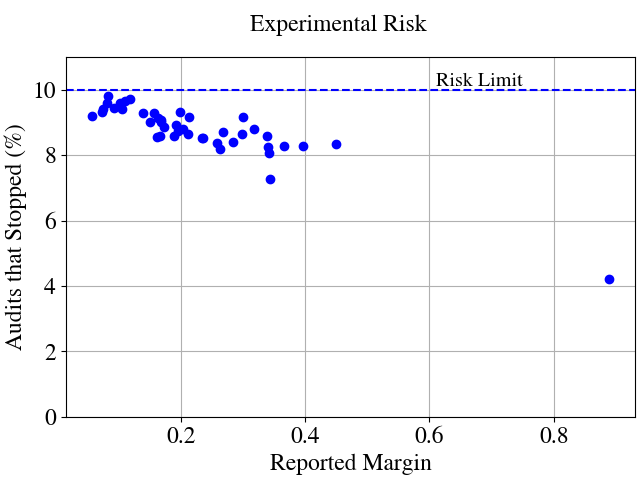
\includegraphics[width=.5\textwidth]{prov_risk.png}
\caption{The fraction of simulated \Providence audits on tied elections that stopped in any rounds (we performed five rounds at a risk limit of $0.1$) as a function of contest margin. This value is an estimate of the maximum risk of the \Providence audit.}
\label{fig:prov-risk}
\end{figure}

In the simulations of \Providence audits of a tied election, the fraction of audits that stop, as shown in Figure~\ref{fig:prov-risk}, is an estimate of maximum risk. For all margins, this estimated maximum risk is less than the risk limit, supporting the claim that \Providence is risk-limiting.

\begin{figure}
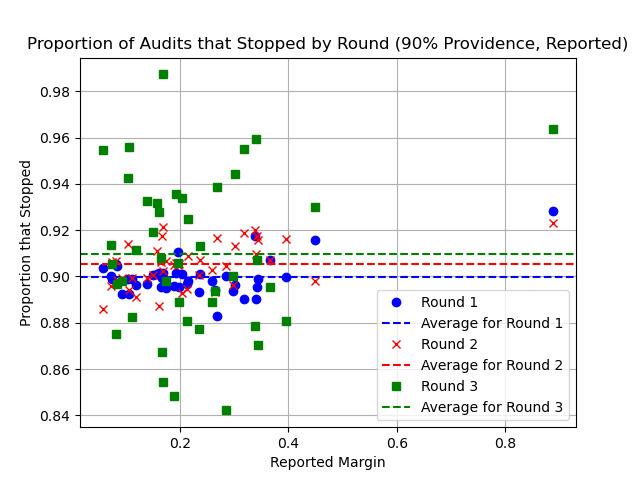
\includegraphics[width=.5\textwidth]{prov_sprob.png}
\caption{The fraction of simulated \Providence audits of the election as reported that stopped for each round as a function of margin. This value is an estimate of the stopping probability conditioned on the sample of the previous round. The average fraction for rounds 1, 2, and 3 is $0.8996$, $0.9052$, and $0.9098$ respectively. We show only the first three rounds since so few audits make it to rounds 4 and 5 (of the order of $10^4 \times (0.1)^3$ and $10^4 \times (0.1)^4$ respectively).}
\label{fig:prov-sprob}
\end{figure}

Simulations of audits of the election as reported provide insight into stopping probability and number of ballots drawn when the election is as reported. Figure~\ref{fig:prov-sprob} shows that the stopping probabilities over the first rounds are near and slightly above $0.9$ as expected, since our software chose round sizes to give at least a $0.9$ conditional stopping probability. The values are not as tight around $0.9$ for later rounds because fewer audit trials make it to later rounds, and our experimental probability estimates are not as accurate. 

We now investigate the efficiency of \Providence compared to \Minerva, SO \BRAVO, and EoR \BRAVO by taking a single margin as an example: the 2020 US Presidential election in the state of Texas, with margin $0.057$. We run an additional $10^4$ simulations for each of the three other audits on the same underlying election and on a tied election. Both \BRAVO implementations use a conditional stopping probability of $0.9$ for each round, while \Minerva uses a first round size with stopping probability $0.9$ and a multiplier of $1.5$ to obtain subsequent round sizes. Figure~\ref{fig:prov-asn} shows the probability of stopping as a function of the number of ballots sampled, a plot similar to those presented in \cite{simulations}. Points above (higher probability of stopping) and to the left (fewer ballots) represent more efficient audits. As shown, \Providence has comparable efficiency to \Minerva, while both are significantly more efficient than either implementation of \BRAVO. In a contest with a narrow margin (in the 2020 US Presidential election, eight states had margins smaller than $0.03$) the difference in number of ballots sampled could correspond to many days of work which would need to be completed before a certification deadline.
% Section~\ref{sec:workload} discusses workload in more depth.

\begin{figure}
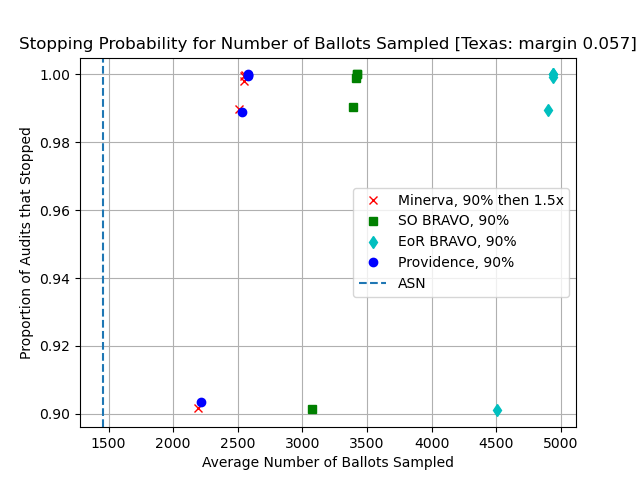
\includegraphics[width=.5\textwidth]{prov_asn.png}
\caption{For the entire audit, consisting of all five rounds, the fraction of simulated audits that stopped as a function of the average number of ballots drawn for \Providence, \Minerva, EoR \BRAVO, and SO \BRAVO. The average sample number (ASN) for \B \BRAVO is included for context.}
\label{fig:prov-asn}
\end{figure}

\newpage






